% Compact bars for Qwen3-8B GPU ForkServe+ and control-plane APP.
% Units: peak KV tokens, decode tokens /1000, e2e seconds, fan-out ms.
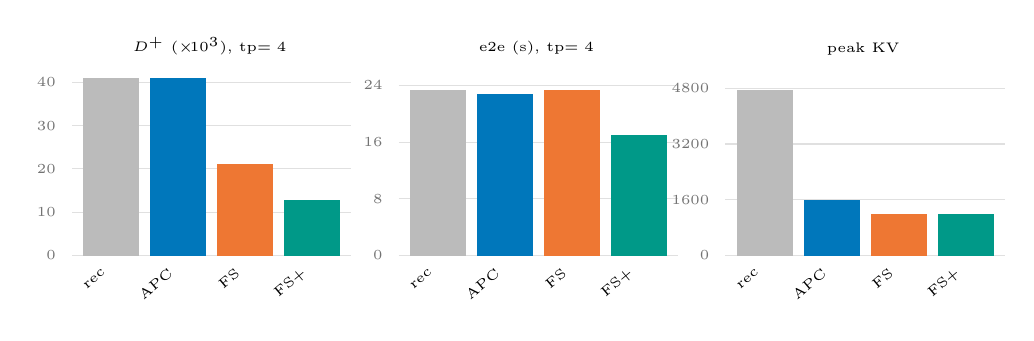
\begin{tikzpicture}[
  font=\scriptsize\sffamily,
  bar/.style={draw=black, line width=0.25pt},
]
\definecolor{Rec}{HTML}{BBBBBB}
\definecolor{APC}{HTML}{0077BB}
\definecolor{FS}{HTML}{EE7733}
\definecolor{FSp}{HTML}{009988}

% ---- left: GSM8K decode tokens (x1000), tp=4 ----
\begin{scope}[shift={(0,0)}]
  \foreach \y in {0,10,20,30,40} {
    \draw[black!12] (0,\y*0.055) -- (3.55,\y*0.055);
    \node[font=\tiny, text=black!55, anchor=east] at (-0.08,\y*0.055) {\y};
  }
  \fill[bar, Rec] (0.15,0) rectangle (0.85,40.96*0.055);
  \fill[bar, APC] (1.00,0) rectangle (1.70,40.96*0.055);
  \fill[bar, FS]  (1.85,0) rectangle (2.55,20.997*0.055);
  \fill[bar, FSp] (2.70,0) rectangle (3.40,12.826*0.055);
  \node[font=\tiny, rotate=40, anchor=east] at (0.50,-0.12) {rec};
  \node[font=\tiny, rotate=40, anchor=east] at (1.35,-0.12) {APC};
  \node[font=\tiny, rotate=40, anchor=east] at (2.20,-0.12) {FS};
  \node[font=\tiny, rotate=40, anchor=east] at (3.05,-0.12) {FS+};
  \node[font=\tiny, anchor=south] at (1.75,2.42) {$D^{+}$ ($\times\!10^{3}$), tp$=4$};
\end{scope}

% ---- middle: GSM8K e2e seconds, tp=4 ----
\begin{scope}[shift={(4.15,0)}]
  \foreach \y in {0,8,16,24} {
    \draw[black!12] (0,\y*0.09) -- (3.55,\y*0.09);
    \node[font=\tiny, text=black!55, anchor=east] at (-0.08,\y*0.09) {\y};
  }
  \fill[bar, Rec] (0.15,0) rectangle (0.85,23.36*0.09);
  \fill[bar, APC] (1.00,0) rectangle (1.70,22.72*0.09);
  \fill[bar, FS]  (1.85,0) rectangle (2.55,23.30*0.09);
  \fill[bar, FSp] (2.70,0) rectangle (3.40,16.94*0.09);
  \node[font=\tiny, rotate=40, anchor=east] at (0.50,-0.12) {rec};
  \node[font=\tiny, rotate=40, anchor=east] at (1.35,-0.12) {APC};
  \node[font=\tiny, rotate=40, anchor=east] at (2.20,-0.12) {FS};
  \node[font=\tiny, rotate=40, anchor=east] at (3.05,-0.12) {FS+};
  \node[font=\tiny, anchor=south] at (1.75,2.42) {e2e (s), tp$=4$};
\end{scope}

% ---- right: peak KV, GSM8K ----
\begin{scope}[shift={(8.30,0)}]
  \foreach \y in {0,1600,3200,4800} {
    \draw[black!12] (0,\y*0.00045) -- (3.55,\y*0.00045);
    \node[font=\tiny, text=black!55, anchor=east] at (-0.08,\y*0.00045) {\y};
  }
  \fill[bar, Rec] (0.15,0) rectangle (0.85,4744*0.00045);
  \fill[bar, APC] (1.00,0) rectangle (1.70,1582*0.00045);
  \fill[bar, FS]  (1.85,0) rectangle (2.55,1182*0.00045);
  \fill[bar, FSp] (2.70,0) rectangle (3.40,1182*0.00045);
  \node[font=\tiny, rotate=40, anchor=east] at (0.50,-0.12) {rec};
  \node[font=\tiny, rotate=40, anchor=east] at (1.35,-0.12) {APC};
  \node[font=\tiny, rotate=40, anchor=east] at (2.20,-0.12) {FS};
  \node[font=\tiny, rotate=40, anchor=east] at (3.05,-0.12) {FS+};
  \node[font=\tiny, anchor=south] at (1.75,2.42) {peak KV};
\end{scope}
\end{tikzpicture}
